% 
\section{Resultados y discusión}
\subsection{Convergencia}
Para revisar la convergencia se usaron las trazas de cada parámetro, la
autocorrelación, la media acumulada por cadena y dos diagnósticos numéricos: el
$\hat{R}$, que compara la variación entre cadenas con la variación dentro de
cada una, y el tamaño de muestra efectivo (ESS). Se tomaron como criterios
$\hat{R}\leq1.01$ y un ESS de al menos 400 en todos los parámetros.

En la base sin duplicados todos los parámetros cumplen ambos criterios
(Tabla~\ref{tab:convergencia}): el $\hat{R}$ está entre $1.00$ y $1.01$ y el ESS
\emph{bulk} va de 1.003 (BS) a 2.195 (HeartRate), con un ESS de colas mínimo de
1.827. En la base con duplicados ocurre lo mismo, con un ESS \emph{bulk} mínimo
de 871, también para BS. Las cuatro cadenas se superponen en las trazas y la
media acumulada de cada una se estabiliza después del \emph{burn-in} en valores
muy cercanos entre cadenas (Figura~\ref{fig:media_acumulada}); las pequeñas
diferencias que se ven en la edad y la frecuencia cardíaca son mínimas frente a
la desviación de su posterior. Por esto se concluye que las cadenas convergen y
que el número de muestras es suficiente para resumir la posterior.

\begin{table}[h]
\centering
\caption{Diagnósticos de convergencia por parámetro.}
\label{tab:convergencia}
\small
\begin{tabular}{lcccc}
\toprule
 & \multicolumn{2}{c}{Sin duplicados} & \multicolumn{2}{c}{Con duplicados}\\
\cmidrule(lr){2-3}\cmidrule(lr){4-5}
Parámetro & $\hat{R}$ & ESS & $\hat{R}$ & ESS\\
\midrule
$\alpha_1$  & 1.00 & 1366 & 1.01 & 1091\\
$\alpha_2$  & 1.01 & 1282 & 1.00 & 1035\\
Age         & 1.00 & 1809 & 1.00 & 1520\\
SystolicBP  & 1.01 & 1197 & 1.00 & 1233\\
DiastolicBP & 1.00 & 2035 & 1.00 & 1843\\
BS          & 1.00 & 1003 & 1.00 & 871\\
BodyTemp    & 1.00 & 1681 & 1.00 & 1626\\
HeartRate   & 1.00 & 2195 & 1.00 & 2123\\
\bottomrule
\end{tabular}
\end{table}

\begin{figure*}[t]
\centering
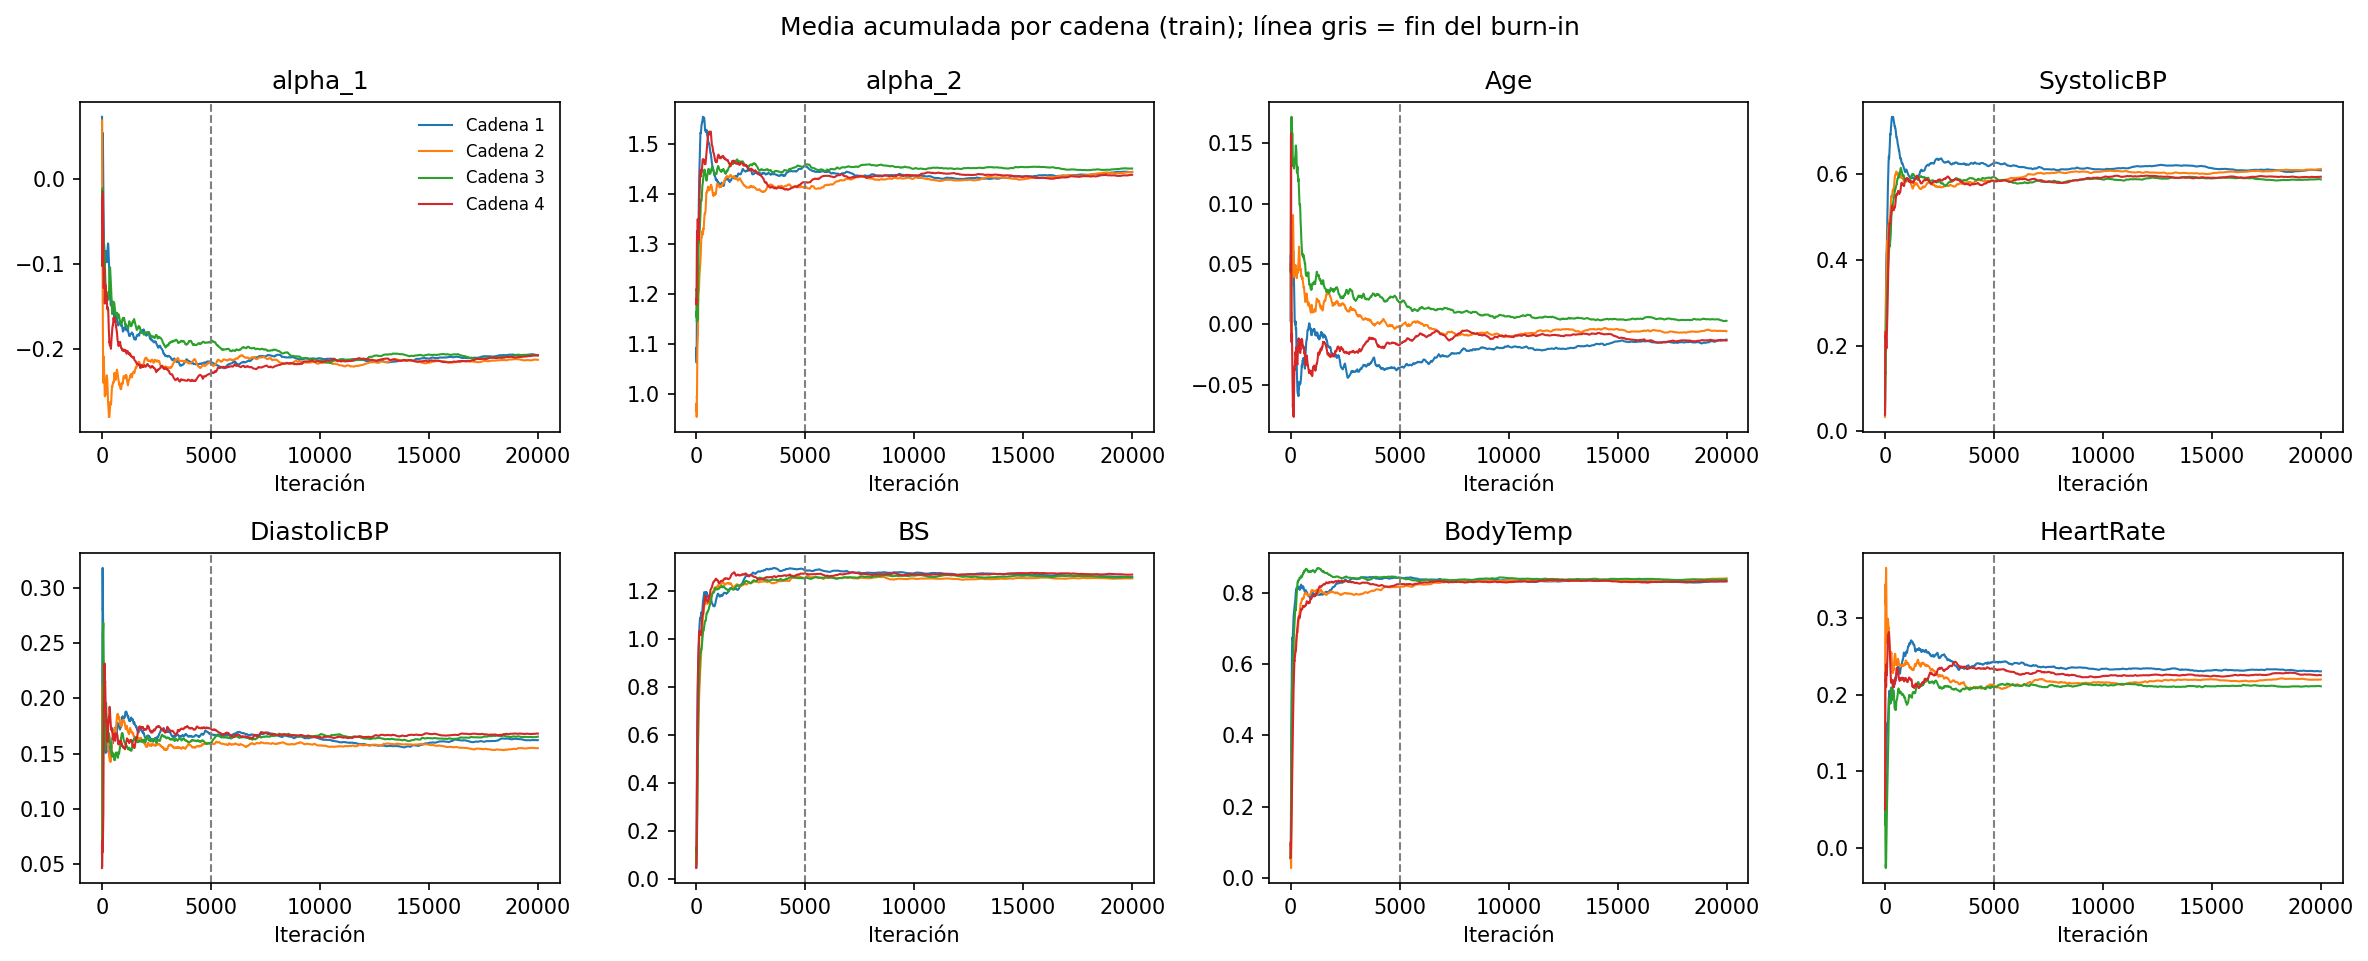
\includegraphics[width=\textwidth]{conv_media_acumulada_train.png}
\caption{Media acumulada de cada parámetro por cadena (base sin duplicados). La línea gris marca el fin del \emph{burn-in}.}
\label{fig:media_acumulada}
\end{figure*}

La comparación entre prior y posterior (Figura~\ref{fig:prior_posterior})
muestra que, para la mayoría de parámetros, la posterior es mucho más angosta
que la prior, es decir, los datos dominan el resultado. Hay dos casos que vale
la pena señalar. En la edad, la prior estaba centrada cerca de $0.4$, pero la
posterior queda alrededor de cero, de modo que los datos contradicen lo que se
esperaba. En la presión diastólica, la posterior se acumula cerca de cero, que
es el límite de su prior truncada.

\begin{figure*}[t]
\centering
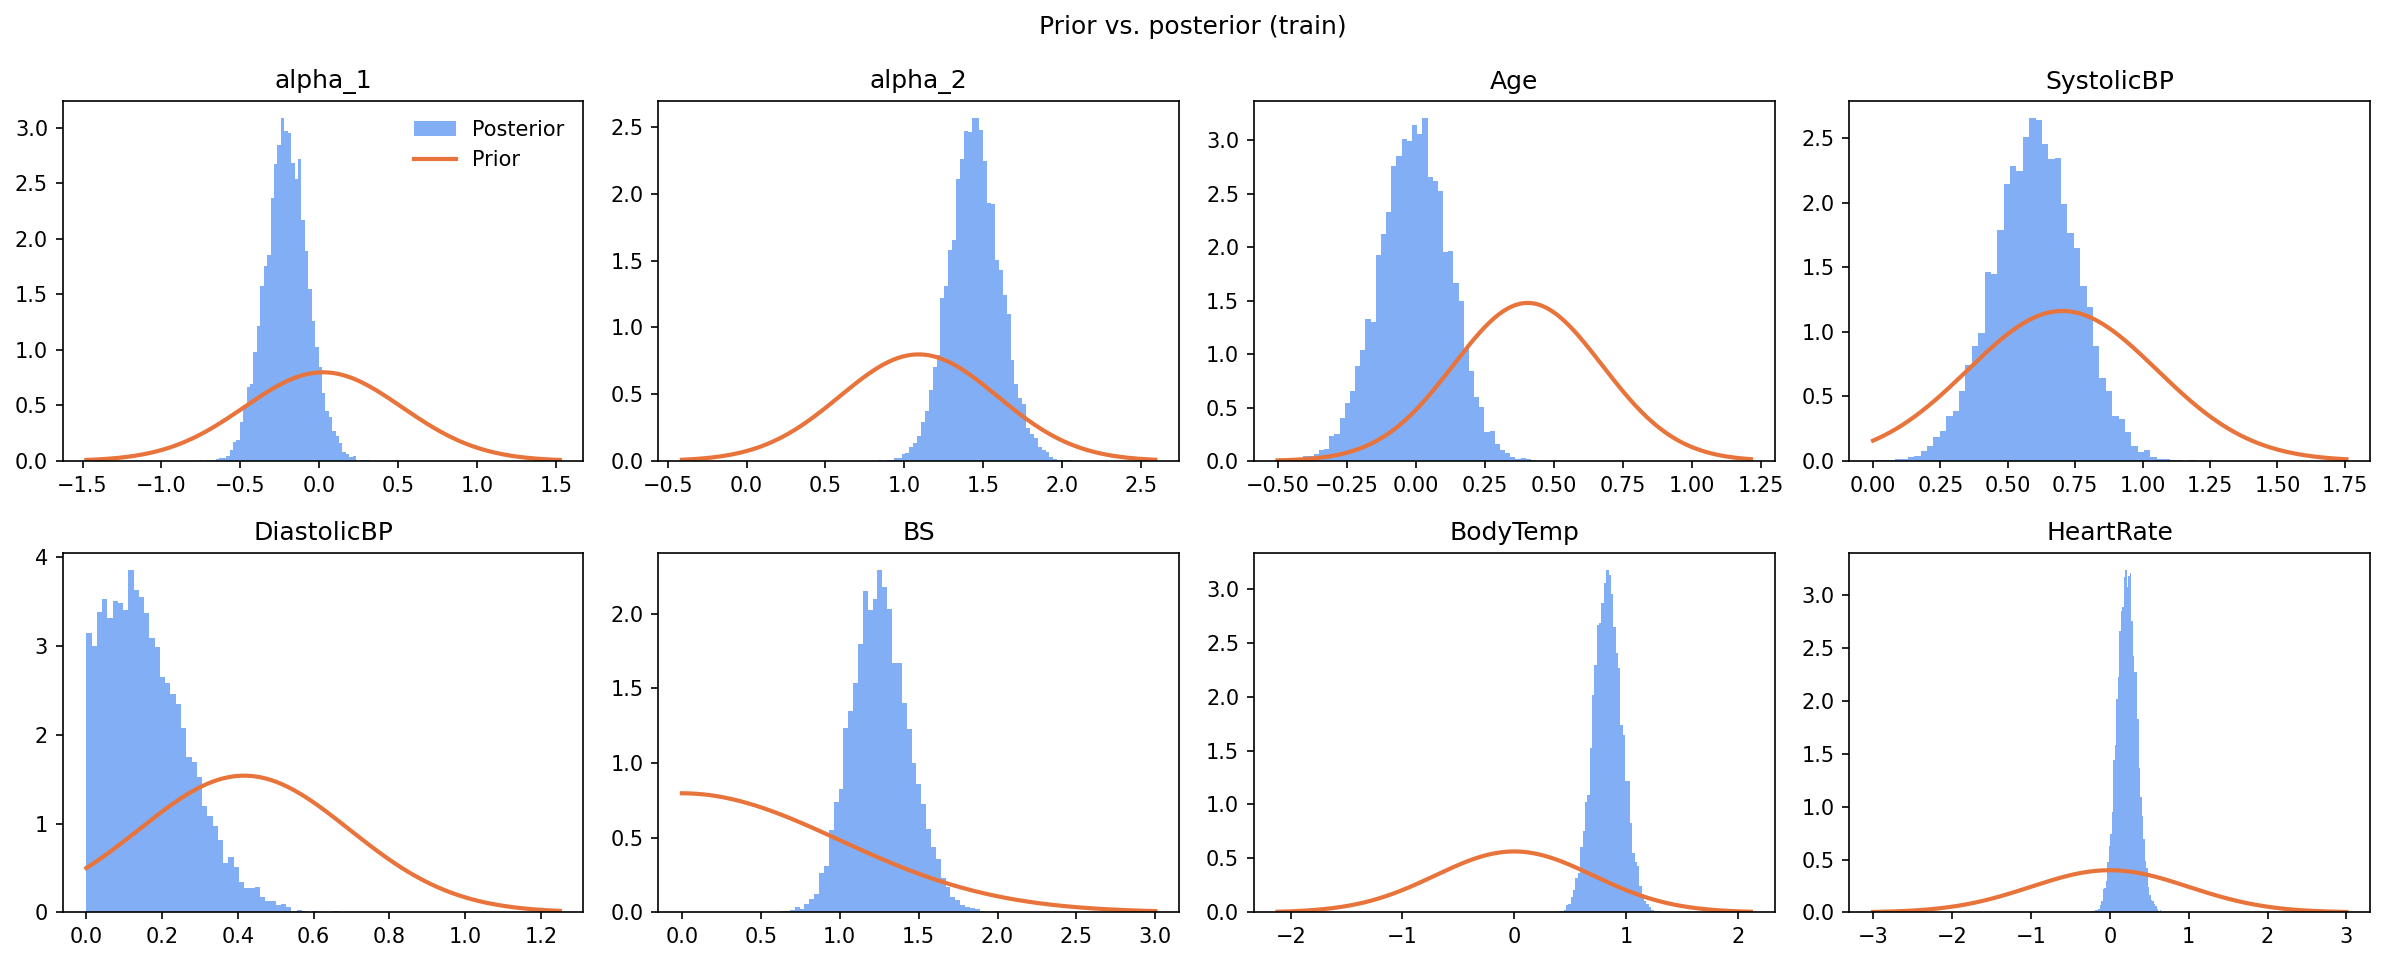
\includegraphics[width=\textwidth]{conv_prior_posterior_train.png}
\caption{Prior (línea) y posterior (histograma) de cada parámetro, base sin duplicados.}
\label{fig:prior_posterior}
\end{figure*}

\begin{table}[h]
\centering
\caption{Resumen de la posterior: media e intervalo de credibilidad del 95\,\%.}
\label{tab:posterior}
\small
\begin{tabular}{lcc}
\toprule
Parámetro & Sin duplicados & Con duplicados\\
\midrule
$\alpha_1$  & $-0.21$ [$-0.47$, $0.07$] & $-0.92$ [$-1.11$, $-0.73$]\\
$\alpha_2$  & $1.45$ [$1.14$, $1.77$]   & $1.23$ [$1.02$, $1.44$]\\
Age         & $-0.01$ [$-0.26$, $0.24$] & $-0.07$ [$-0.25$, $0.11$]\\
SystolicBP  & $0.60$ [$0.29$, $0.90$]   & $0.78$ [$0.56$, $0.99$]\\
DiastolicBP & $0.16$ [$0.01$, $0.41$]   & $0.13$ [$0.01$, $0.31$]\\
BS          & $1.26$ [$0.92$, $1.63$]   & $1.49$ [$1.23$, $1.77$]\\
BodyTemp    & $0.84$ [$0.59$, $1.10$]   & $0.74$ [$0.58$, $0.91$]\\
HeartRate   & $0.22$ [$-0.02$, $0.46$]  & $0.34$ [$0.17$, $0.49$]\\
\bottomrule
\end{tabular}
\end{table}

\subsection{Validación con la base de prueba}
Para cada gestante del conjunto de prueba se calcularon las probabilidades de
las tres clases con cada muestra de la posterior y se promediaron, obteniendo
su probabilidad predictiva. A partir de esas probabilidades se compararon dos
formas de clasificar. La primera es la regla MAP, que asigna la clase más
probable. La segunda es una regla de costo esperado, que asigna la clase con
menor costo según una matriz que sigue el orden de gravedad de los errores
definido en el planteamiento del problema: lo más grave es clasificar como bajo
a una gestante de alto riesgo, le sigue clasificarla como medio, y lo menos
grave es la falsa alarma. La matriz usada, con filas para la clase real y
columnas para la predicha (bajo, medio, alto), es
\[
C=\begin{pmatrix}0&1&2\\2&0&1\\6&3&0\end{pmatrix}.
\]
La incertidumbre de cada métrica se obtuvo calculándola con cada muestra de la
posterior y tomando los percentiles 2.5 y 97.5.

\begin{table}[h]
\centering
\caption{Métricas en la base de prueba sin duplicados ($n=117$).}
\label{tab:metricas}
\small
\begin{tabular}{lcc}
\toprule
Métrica & Costo esperado [IC 95\,\%] & MAP\\
\midrule
Recall alto riesgo  & $0.86$ [$0.75$, $0.93$] & $0.68$\\
Recall riesgo medio & $0.40$ [$0.20$, $0.56$] & $0.04$\\
MCC                 & $0.38$ [$0.30$, $0.41$] & $0.43$\\
Exactitud balanceada& $0.60$ [$0.54$, $0.63$] & $0.55$\\
Exactitud           & $0.59$ [$0.54$, $0.60$] & $0.68$\\
\bottomrule
\end{tabular}
\end{table}

Con la regla MAP el modelo prácticamente no predice la clase de riesgo medio
(recall de $0.04$): las gestantes de esa clase terminan clasificadas como de
riesgo bajo o alto. Esto se debe a que en ninguna gestante la probabilidad de
riesgo medio supera $0.39$, por lo que nunca es la clase más probable. También
se probó una regla que asigna alto riesgo cuando su probabilidad supera un
umbral; con umbrales entre $0.20$ y $0.50$ el recall de alto riesgo va de $0.89$
a $0.68$, pero el de riesgo medio se mantiene entre $0$ y $0.08$, de modo que
mover el umbral no resuelve el problema de la clase media.

La regla de costo esperado sí lo hace, porque usa las tres probabilidades y no
solo la más alta: recupera la clase media (recall de $0.40$) y sube el recall de
alto riesgo de $0.68$ a $0.86$, con la mejor exactitud balanceada ($0.60$). El
precio es un mayor número de falsas alarmas en las gestantes de riesgo bajo, que
es justamente el error que se definió como menos grave, y por eso el MCC y la
exactitud global son algo menores que con la regla MAP (Figura~\ref{fig:confusion}).
Por coherencia con el objetivo del proyecto, que prioriza detectar a las
gestantes de alto riesgo, se toma la regla de costo esperado como regla principal.

\begin{figure}[h]
\centering
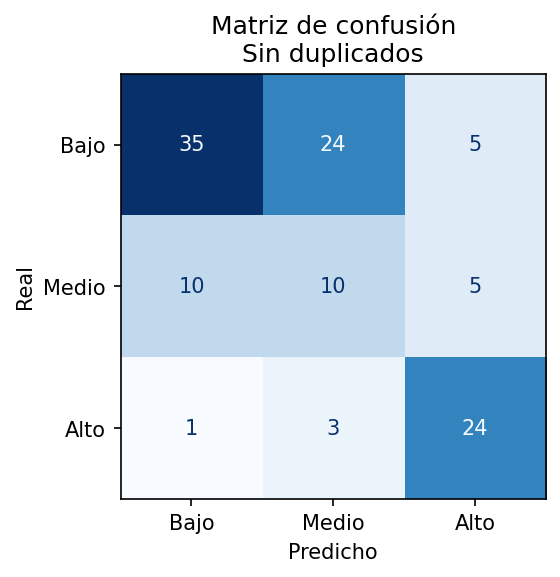
\includegraphics[width=0.49\columnwidth]{eval_confusion_train.png}
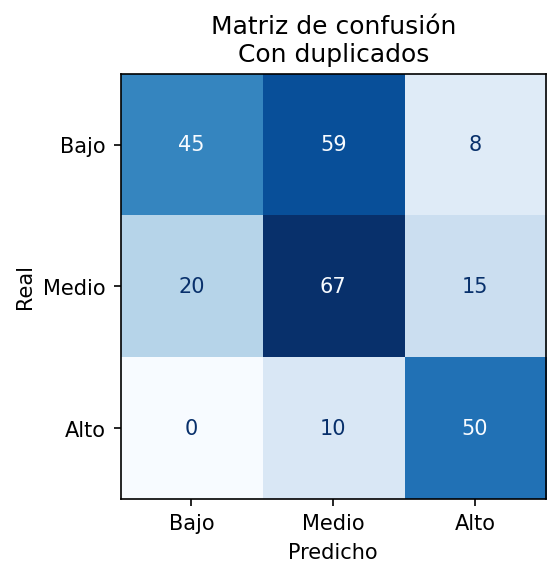
\includegraphics[width=0.49\columnwidth]{eval_confusion_train_full.png}
\caption{Matrices de confusión con la regla de costo esperado: sin duplicados (izq.) y con duplicados (der.).}
\label{fig:confusion}
\end{figure}

\subsection{Respuesta a la pregunta de investigación}
Las variables fisiológicas registradas permiten clasificar el nivel de riesgo de
forma moderada. Con la regla de costo esperado, el modelo detecta 86\,\% de las
gestantes de alto riesgo, con una exactitud balanceada de $0.60$ y un MCC de
$0.38$, pero distingue mal la clase de riesgo medio, que es la más pequeña y la
que más se traslapa con las otras dos.

En cuanto al peso predictivo, y como todas las variables están en la misma
escala, los coeficientes se pueden comparar directamente. La glucemia (BS) es
la variable de mayor peso: un aumento de una desviación estándar multiplica por
cerca de $3.5$ las odds de pasar a un nivel de riesgo mayor. Le siguen la
temperatura corporal ($2.3$) y la presión sistólica ($1.8$), las tres con
intervalos lejos de cero. La frecuencia cardíaca ($1.25$) y la presión
diastólica ($1.18$) tienen un efecto pequeño, y la edad no muestra efecto
($0.99$, con un intervalo centrado en cero).

\subsection{Discusión}
Al comparar con la base con duplicados, el orden de importancia de las variables
se mantiene, con BS, la presión sistólica y la temperatura como las de mayor
peso, y la edad sin efecto. Lo que cambia es la incertidumbre: con duplicados
los intervalos de credibilidad son más angostos, porque cada copia cuenta como
una observación nueva en la likelihood y la posterior parece más precisa de lo
que realmente es. Los puntos de corte también cambian, ya que las proporciones
de las clases son distintas en esa base. En la validación, el recall de alto
riesgo es parecido en ambas ($0.86$ frente a $0.83$), por lo que tener más filas
repetidas no mejora la detección de los casos más graves; además, en la base
con duplicados el conjunto de prueba también repite registros, lo que hace que
sus métricas no sean directamente comparables. Esto respalda la decisión de
trabajar con los registros únicos.

Entre las limitaciones, la principal es la clase de riesgo medio. El modelo
asume odds proporcionales, es decir, un mismo efecto de cada variable en los
dos puntos de corte, y la dificultad para separar esa clase sugiere que este
supuesto no se cumple del todo con estos datos. El resultado de la edad apunta
en la misma dirección: el riesgo aumenta tanto en edades muy bajas como muy
altas, y una relación lineal no capta ese comportamiento. Por otro lado, la
matriz de costos es una decisión del grupo basada en el orden de gravedad de los
errores, no un valor clínico validado, y el conjunto de prueba es pequeño (117
registros), lo que explica la amplitud de algunos intervalos. Finalmente, la
fuente no documenta cómo se asignó la etiqueta de riesgo, por lo que el modelo
aprende a reproducir esa etiqueta y no necesariamente un criterio clínico.
